\section{Trajectoire de migration et gouvernance}
\label{sec:trajectoire}

\subsection{Paliers}
La cible ne se déploie pas d'un bloc. La figure~\ref{fig:trajectoire} propose trois paliers successifs, chacun livrant une valeur mesurable et conservant la continuité du service~:
\begin{description}
  \item[Palier 1 -- Socle (2027)] mise en place du moteur de processus, de la passerelle d'API et du bus d'événements~; raccordement de l'e-timbre et de l'état civil~; premier service d'IA (contrôle documentaire) en mode assistance à l'agent, puis en mode automatique après mesure de sa fiabilité~; création du back-office d'instruction. Résultat attendu~: suppression du formulaire papier et division par deux des dossiers incomplets au guichet.
  \item[Palier 2 -- Étendu (2028)] application mobile «~Mon e-ID~» unifiant carte numérique et demandes~; assistant conversationnel~; prévision d'affluence et créneaux recommandés~; livraison à domicile~; tableaux de bord. Résultat attendu~: canal mobile majoritaire, temps en centre inférieur à quinze minutes.
  \item[Palier 3 -- Cible (2030)] renouvellement entièrement en ligne pour les porteurs dont la biométrie de référence est récente, détection d'anomalies et pilotage prédictif, gouvernance MLOps complète, interconnexion au Registre National de la Population. Résultat attendu~: objectifs G1 à G5 atteints.
\end{description}

\begin{figure}[h]
\centering
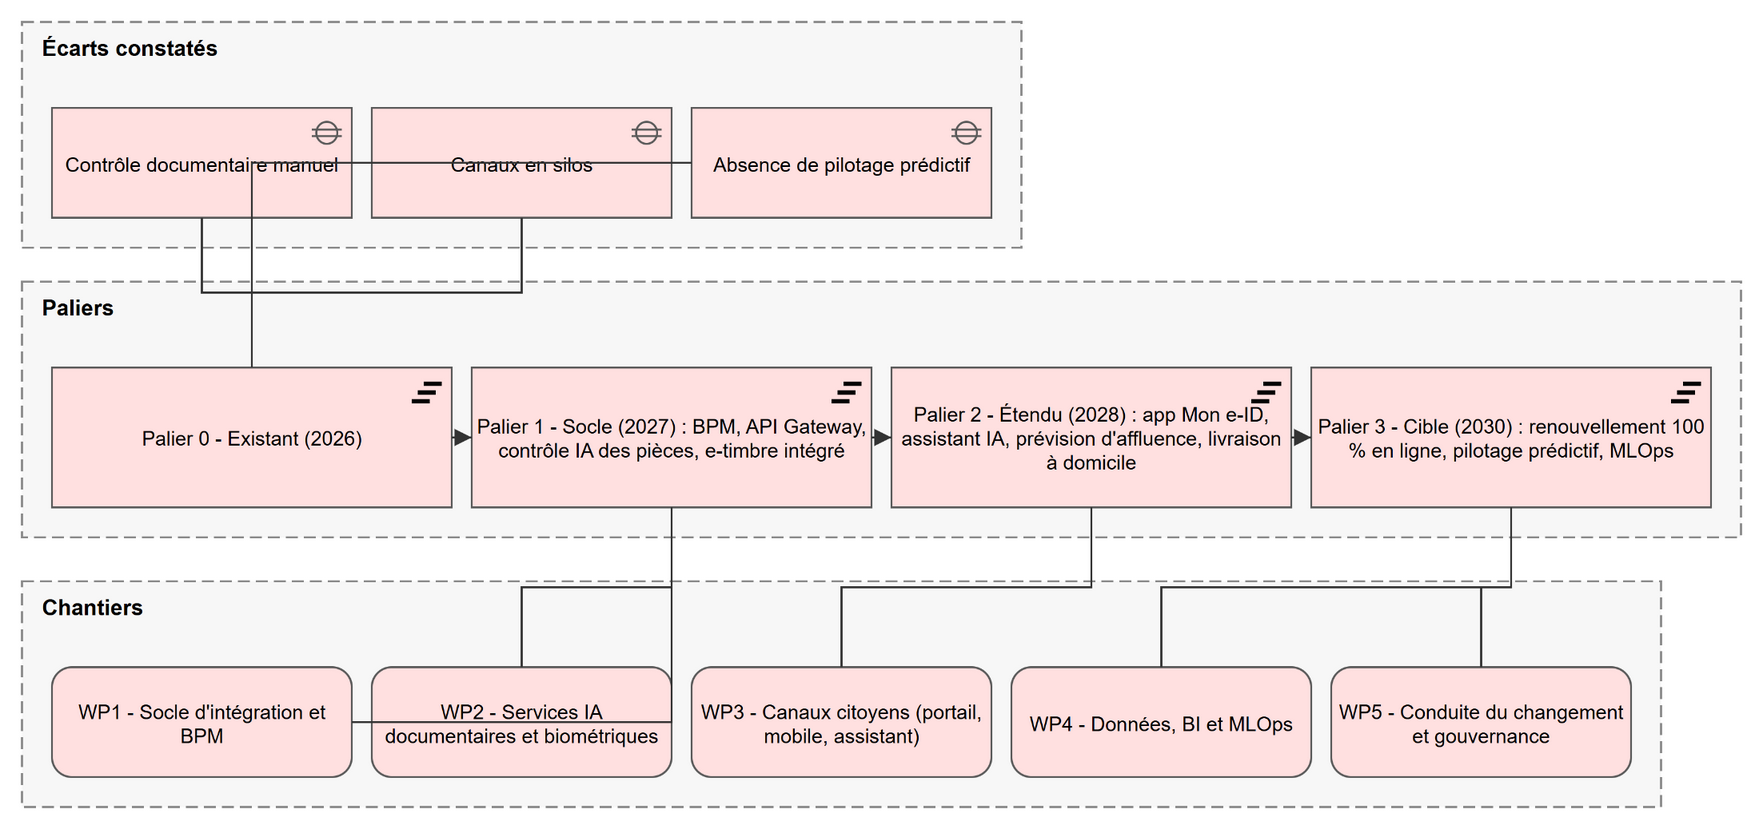
\includegraphics[width=\columnwidth]{archimate/V6_trajectoire.png}
\caption{Trajectoire de migration~: écarts, paliers et chantiers (ArchiMate, couche implémentation et migration).}
\label{fig:trajectoire}
\end{figure}

\subsection{Chantiers et gouvernance}
Cinq chantiers portent la trajectoire~: socle d'intégration et BPM~; services d'IA documentaires et biométriques~; canaux citoyens~; données, BI et MLOps~; conduite du changement et gouvernance. Ce dernier chantier est décisif~: formation des agents des CEDI au nouveau rôle d'accueil, création du métier d'instructeur, communication vers les citoyens, et instauration d'un \emph{comité d'architecture} qui valide chaque évolution au regard des principes d'urbanisation, tient à jour les cartographies et arbitre la dette technique. Un \emph{comité d'éthique de l'IA}, associant la CNDP, examine chaque modèle avant sa mise en service et revoit périodiquement ses indicateurs d'équité.

\subsection{Risques du programme}
\begin{table}[h]
\caption{Principaux risques du programme et parades}
\label{tab:risques}
\centering
\small
\begin{tabularx}{\columnwidth}{XX}
\toprule
\textbf{Risque} & \textbf{Parade} \\
\midrule
Rejet par les agents d'un contrôle automatique perçu comme concurrent & Déploiement en mode assistance d'abord, indicateurs partagés, valorisation du rôle d'instructeur \\
Fracture numérique et exclusion & Maintien du guichet, assistance en centre, assistant vocal multilingue, cas particuliers à domicile \\
Faux rejets du contrôle documentaire & Seuils prudents, instruction humaine systématique de la zone de doute, mesure continue \\
Dépendance à un fournisseur d'IA & Modèles hébergés sur site, formats ouverts, compétences internes \\
Dérive du périmètre & Paliers à valeur mesurable, comité d'architecture, gel des évolutions hors cartographie \\
\bottomrule
\end{tabularx}
\end{table}
